% -*- root: ../main.tex -*-

% Devono essere esposte le scelte progettuali operate nelle varie fasi di sviluppo dell'elaborato. In questa sezione devono essere documentati gli schemi di progetto relativamente all'architettura complessiva del sistema e alle sue componenti di rilievo che possano meritare un'analisi di dettaglio. Per le componenti software si può ricorrere ad esempio a diagrammi delle classi, di sequenza, stato, attività. Per le componenti hardware è possibile includere opportuni schemi in grado di descrivere l'architettura fisica adottata.
% 15000 - 24000 battute 

%Architettura complessiva, descrizione di pattern architetturali usati, componenti del sistema distribuito, scelte tecnologiche cruciali ai fini architetturali -- corredato da pochi ma efficaci diagrammi
%Ricordate che una scelta architetturale può ritenersi giustificata o meno solo a fronte dei requirement che avete indicato; viceversa, ogni requirement "critico" dovrebbe influenzare qualcuna della scelte architetturali effettuate e descritte.
%L'architettura deve spiegare quali sono i sotto-componenti del sistema (da 5 a 15, diciamo), ognuno cosa fa, chi parla con chi e per dirsi cosa -- i diagrammi aiutano, ma poi la prosa deve chiaramente indicare questi aspetti.
\chapter{Design Architetturale}
    ...
    \section{Architettura Generale}
    Inserimento del diagramma delle classi generale in cui si vedono le interazioni tra Model View e Controller
    
    \begin{figure}[H]
        \centering
        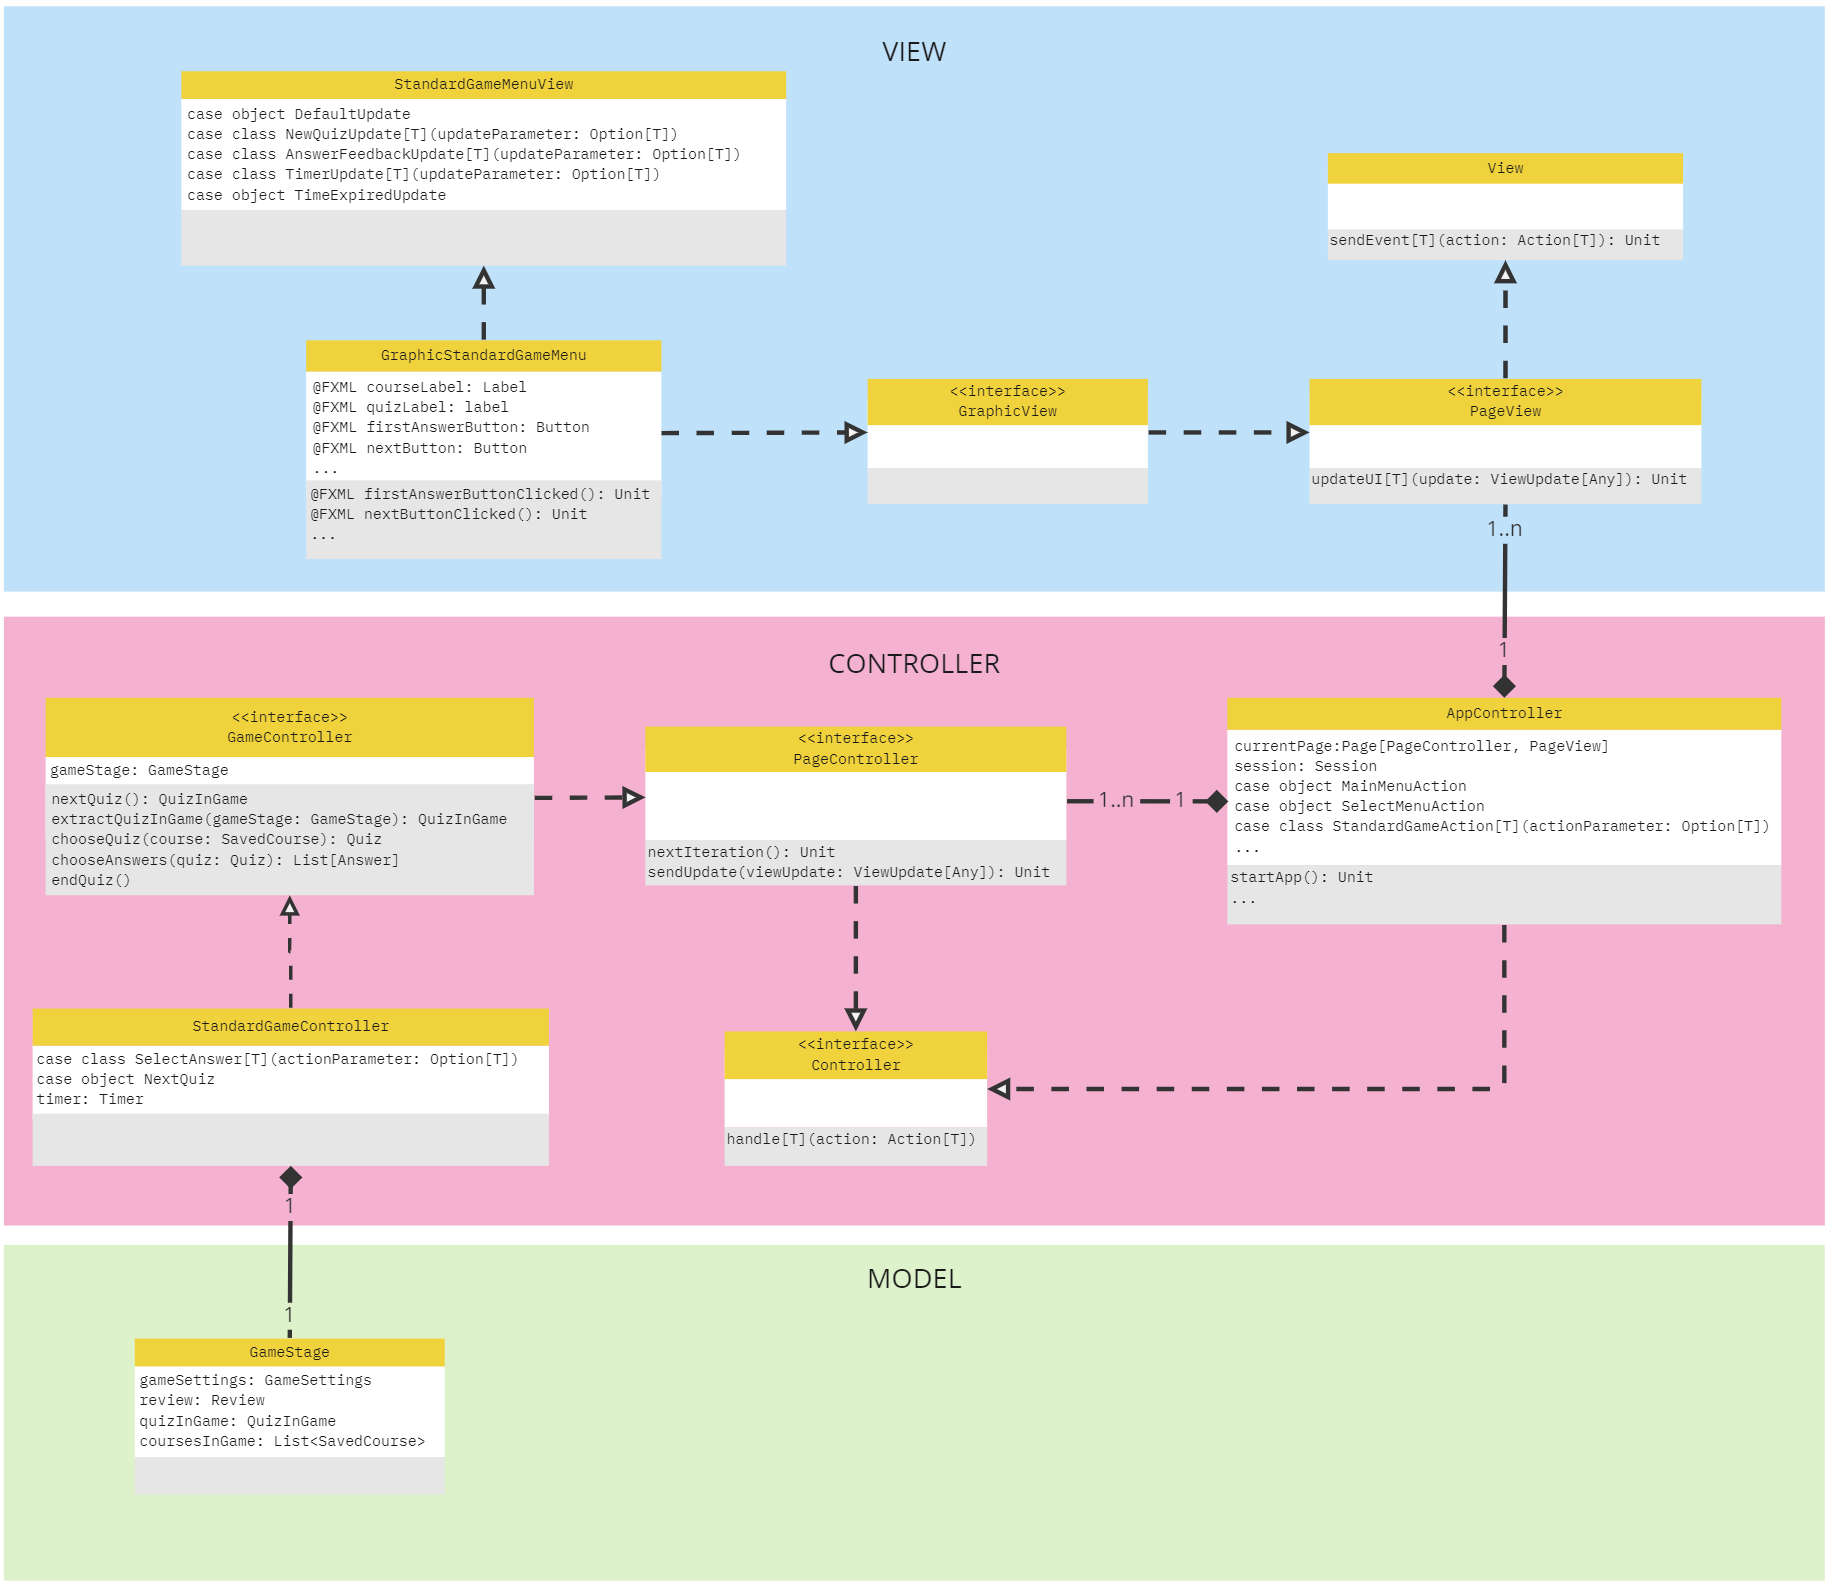
\includegraphics[width=\textwidth]{Miro/general_architecture.png}
        \label{fig:Sprint9BL2}
    \end{figure}
    
    \section{Pattern Architetturali Utilizzati}
        Nel sistema è stato utilizzato il pattern Model View Controller (MVC) in modo da modularizzare quanto più possibile le parti relative all'interfaccia grafica, la modellazione e la logica dell'applicazione. 
        Questo pattern è stato utile considerando anche la metodologia di sviluppo agile per realizzare versioni successive del sistema implementando, ad esempio, un'interfaccia basata su linea di comando nelle prime fasi del progetto e poi una interfaccia che utilizzasse JavaFX nelle fasi successive di sviluppo.
        
        Il funzionamento del pattern MVC è il seguente:
        \begin{itemize}
            \item Il Model fornisce i metodi per accedere ai dati;
            \item La View si occupa di interagire con l'utente, notificare il Controller e visualizzare i dati del Model;
            \item Il Controller riceve i comandi dell'utente e si occupa di aggiornare lo stato della View e del Model.
        \end{itemize}
    